% Ajustar esse \vspace de acordo com o necessário
\vspace{-42pt}

O projeto terá uma parte de hadware e de software. Na parte de hardware será utilizado:
\begin{itemize}
   \item O servidor do LCEE que fará a armazenagem e processamento de dados; 
   \item Um leitor de código de barras para reconhecer o equipamento e a matrícula na carteirinha;
   \item Componentes elétrônicos e microcontroladores para montar um sistema embarcado para viabilizar a comunicação do leitor de código de barras com o servidor e também para fornecer a localição do equipamentos;
   \item GPS para fornecer a localização geográfica.
\end{itemize}
Já na parte de software será utilizado:
\begin{itemize}
   \item Um Framework PHP como CakePHP para facilitar no desenvolvimento; 
   \item Banco de dados SQL (Structured Query Language).
   \item Pacote XAMPP que apresenta os principais servidores de código aberto do mercado, utilizado para o desenvolvimento da interface WEB.
\end{itemize}

Uma inspiração que temos para software é a plataforma web Lend-Itens mostrado nas figuras \ref{fig:Lend-Itens1} e \ref{fig:Lend-Itens2} que é uma plataforma Web paga para empréstimos de objetos.

\begin{figure}[!h]
	\centering
	\caption{Na plataforma Lend-Itens, os usuários podem acessar sua biblioteca para pesquisar um item e reservá-lo, bem como ver seu histórico e os empréstimos atuais.}
	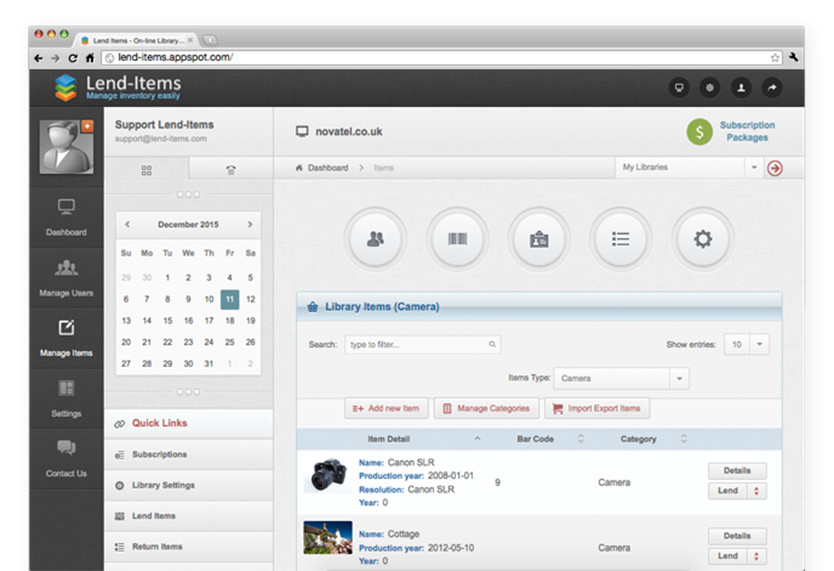
\includegraphics[width=0.7\textwidth]{figura1.jpg}
	\source[\citeonline{LandItens}.]
	\label{fig:Lend-Itens1}
\end{figure}

\begin{figure}[!h]
	\centering
	\caption{Pode-se verificar quais são as pessoas que utilizam a plataforma.}
	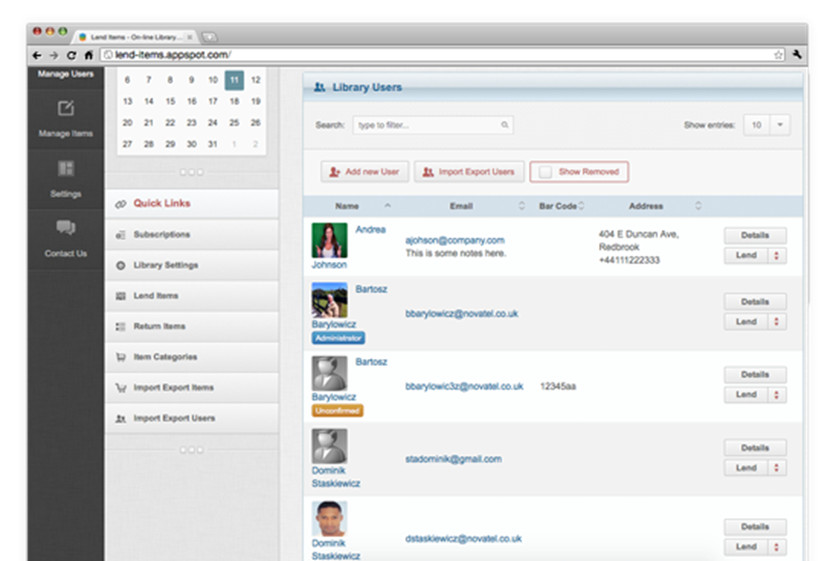
\includegraphics[width=0.7\textwidth]{figura2.jpg}
	\source[\citeonline{LandItens}.]
	\label{fig:Lend-Itens2}
\end{figure}

Há outras plataformas que pode ter como base como Vaivem apresentado na figura \ref{fig:Vaivem}. Há outros softwares também como Software de Controle de UPJ e TotalLoc.

\begin{figure}[!h]
	\centering
	\caption{Interface de Vaivem.}
	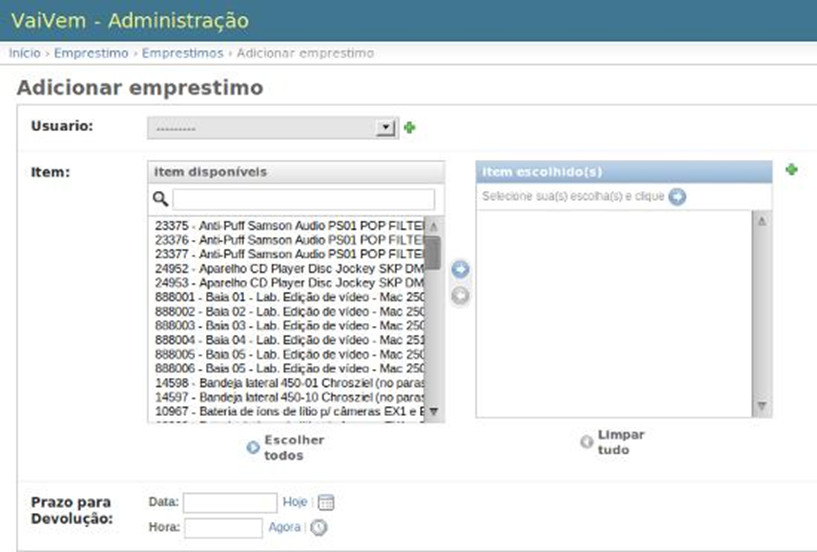
\includegraphics[width=0.7\textwidth]{figura3.jpg}
	\source[\citeonline{SistEmprestimo}.]
	\label{fig:Vaivem}
\end{figure}

Também estamos utilizando o seguinte modelo de banco de dados para nosso projeto :

\begin{figure}[!h]
	\centering
	\caption{Configuração do Banco de Dados.}
	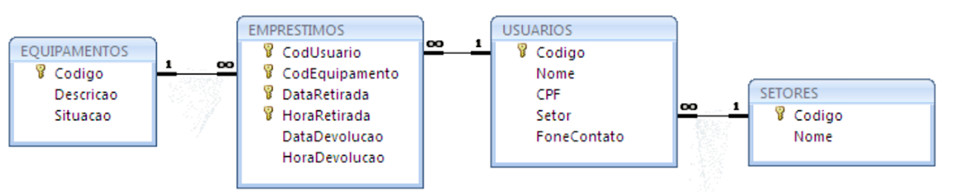
\includegraphics[width=0.7\textwidth]{figura4.jpg}
	\source[\citeonline{DepEngEle}.]
	\label{fig:label_da_figura}
\end{figure}


Também podemos ver quando o banco é acessado pelo seguintes esquemático:

\begin{figure}[!h]
	\centering
	\caption{Acesso do Banco de Dados.}
	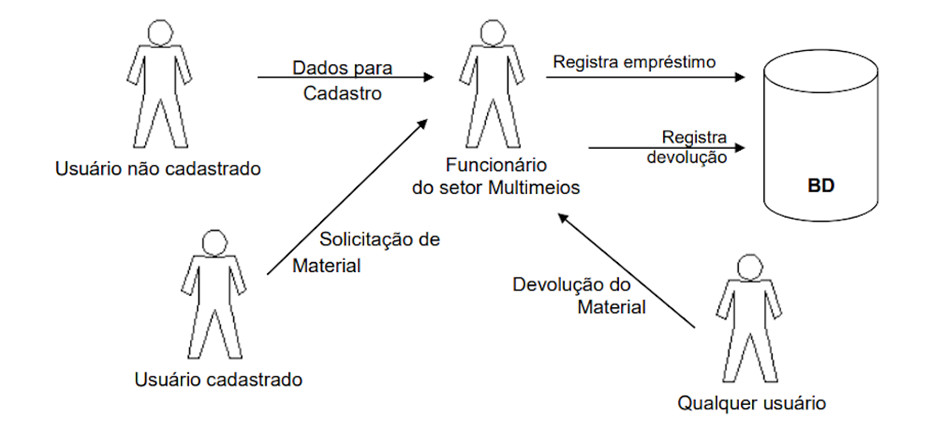
\includegraphics[width=0.7\textwidth]{figura5.jpg}
	\source[\citeonline{DepEngEle}.]
	\label{fig:label_da_figura}
\end{figure}
